\chapter{Methods}

\section{Data representation}

The code used in this project was written in python, using the Numba just-in-time compiler to achieve optimal execution speed (along best practices and algorithm optimizations in writing the code). From a development standpoint, every single Ising model configuration is represented in python as a $d$ dimensional numpy array of shape $N$ repeated $d$ times.

\begin{minted}[linenos, frame=lines]{python}

def new_random_ising(N: tuple[int, ...]):
    return np.ones(N, dtype = np.int8)

m = new_random_ising(tuple([N] * dim))

\end{minted}

[TODO: Fix J, h in the code snippet]

Note that the data type that the numpy array contains is np.int8. In order to minimize storage space, the idea of using boolean variables to represent $1$ and $-1$ was considered, but was ultimately ditched in favour of storing integers. The latter grants faster executions when calculating physical observables (e.g.: energy, magnetization) at the loss of some disk space.

\br

Every one of these numpy array is generated and stored in another numpy array of arbitrary length that represents the Markov Chain. This is done for a number of temperatures around the expected critical temperature, and is repeated for every lattice size under scrutiny and for every dimension. Ultimately, this data is stored in a hdf5 file for efficient i/o operations and in order to contextually add metadata and processed data (e.g.: autocorrelation time, thermalisation time, etc.) to the raw chain.

For every combination of dimension and lattice size, the generated row data is stored in a numpy array of shape ($N_{temps}$, $N_{steps}$, [$N_{dim}$] \times \: $d$).

[TODO: discuss floating point precision, data structures, etc.]

\section{Monte Carlo Markov Chains}

\subsection{Generation}

To study a system at a given temperature it is necessary to be able to generate a random configuration of said system. These random configurations are distributed as a function of their energy: as discussed the probability of a system of being in a state with energy $E$ in the canonical ensemble is given by:

\begin{equation}
	P(E) = \frac{\Omega(E) e^{-\beta E}}{Z}
\end{equation}

Now, it would be ideal to write this probability analytically: to do that we would need to know how to write both $\Omega(E)$ and $Z$, but but such an operation is, unfortunately, simply not possible. The lone computing of $Z$ would require summing over all possible configurations of the system, which in turns would mean to compute the energy of every single configuration. The number of possible configurations of a $(N d)$ spins lattice is $2^{(N d)}$ and computing the energy of a single configuration is an $O(N)$ operation, which means that the overall complexity of computing $Z$ is $\bigO(N 2^{(N d)})$, which is clearly not viable for any reasonable value of $N$.

\br

The solution to this problem is the use of a Markov Chain Monte Carlo method, that is a method for generating a sequence of independent samples from a desired distribution without knowing the normalization constant. One algorithm that produces such a chain is the Metropolis-Hastings algorithm. This algorithm can draw samples from any probability distribution with probability density $P(x)$, provided that we know another function proportional to the density $P$ that we're able to compute analitically (in this case $e^{-\beta E}$) so that we can write $P(E) \propto e^{-\beta E}$.

The algorithm's idea is to start from a random configuration of the system and then to move to a similar configuration with a certain probability linked to the energy distribution.

The formal steps of the Metropolis algorithm in this use case are:

\begin{enumerate}
	\item Start from a random configuration of the system $x$.
	\item Randomly select a spin (or a number of spins) and flip it. We call this new configuration $x'$.
	\item Compute the energy difference of the two systems $\Delta E$.
	\item Set an acceptance probability parameter $\alpha$ based on the energy change and the temperature: $\alpha = \frac{T(x' \to x) P(x')}{T(x \to x') P(x)}$ where $P$ is the Boltzmann distribution. This is the core of the algorithm and it's what allows the Markov Chain to converge to the desired distribution.
	\item Accept the new configuration with probability $\min(1, \alpha)$, otherwise reject it and keep the current configuration. That is, if the new configuration is more probable than the current one, accept it, otherwise accept it with probability $\alpha$ (that is, a probability proportional to the ratio of the two probabilities).
	\item Add the current configuration to the Markov Chain.
	\item Repeat steps 2-6 for a number of iterations. 
\end{enumerate}

Where the "trick" is that computing $\alpha$ both $Z$ and the $\Omega$ terms cancel out.

Note that randomly selecting a spin and flipping it (step 2) is effectively moving to another random configuration of the system close to the current one. This movement is intepreted as a random sample from a distribution centered around the current configuration. Picking a random spin to flip is an arbitrary choice, and other methods could be used to select a neighboring configuration, but has the advantage that the probability of moving from $x$ to $x'$ ($T(x \to x')$) is the same as moving from $x'$ to $x$ ($T(x' \to x)$), which is the Hastings condition of the algorithm. This condition is not striclty necessary, but it simplifies the computation of $\alpha = \frac{e^-\beta E'}{e^{-\beta E}} = e^{-\beta \Delta E}$ to be only dependent on the energy change and the temperature.

\begin{minted}[linenos, frame=lines, breaklines]{python}

def metropolis_hastings(model: np.ndarray, T: float, steps: int):
	'''
	Generate a Markov Chain of configurations of the Ising model at a given temperature T.
	'''

    curr_model = np.copy(model)
    models_samples = np.empty(
		(steps,) + curr_model.shape,
		dtype = curr_model.dtype
	)
    
	N = curr_model.shape[0]
    
    for i in range(steps):
        idx0 = np.random.randint(0, N)
        spin = curr_model[idx0]
        deltaE = compute_energy_change(curr_model, idx0)
        
        accept_probability = np.minimum(1.0, target_distribution(deltaE, T))
        if np.random.random() <= accept_probability:
            curr_model[idx0] = -curr_model[idx0]
        
        models_samples[i] = curr_model
    
    return models_samples

\end{minted}

Also note that since $\alpha$ depends only on the relative energy change the computation can be greatly optimized by computing only the energy change given by the single spin flip, instead of computing the energy of two entire configurations.

[TODO: discuss Metropolis-Hastings algorithm]

% \begin{figure}[htbp]
% 	\centering
% 	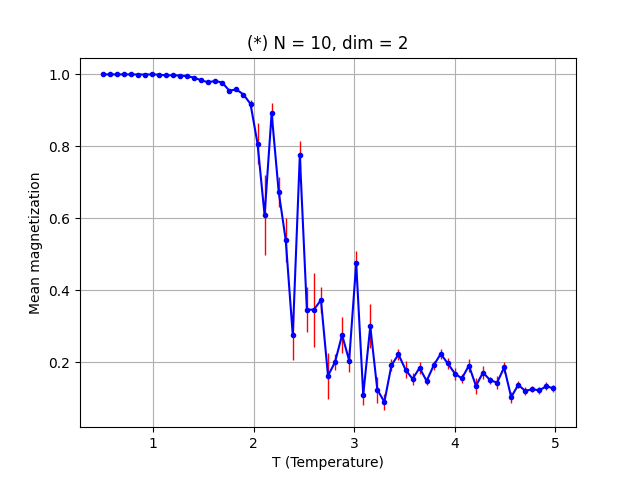
\includegraphics[width=1.\textwidth]{../tmp}
% 	\caption{Markov Chain and relative distribution of the energy of the system.}
% 	\label{figure:markov_chain}
% \end{figure}

\subsection{Analysis}

A Markov Chain is a sequence of random variables where the probability of each variable depends only on the previous variable. This effectively means that even though the sequence of data generated by the Metropolis-Hastings algorithm is distributed according to the Boltzmann distribution the samples are not very useful as a data sample since they are not independent: on the contrary, they are very closely correlated and the presence of correlations between samples would lead to biased results during analysis.

The extraction of decorrelated data is a problem composed of two parts: the thermalisation and the autocorrelation time. The first one is the number of steps that the Markov Chain needs to reach a stationary distribution, while the second one is the number of steps that need to exist between successive samples before they can be considered independent.

\begin{figure}[htbp]
	\centering
	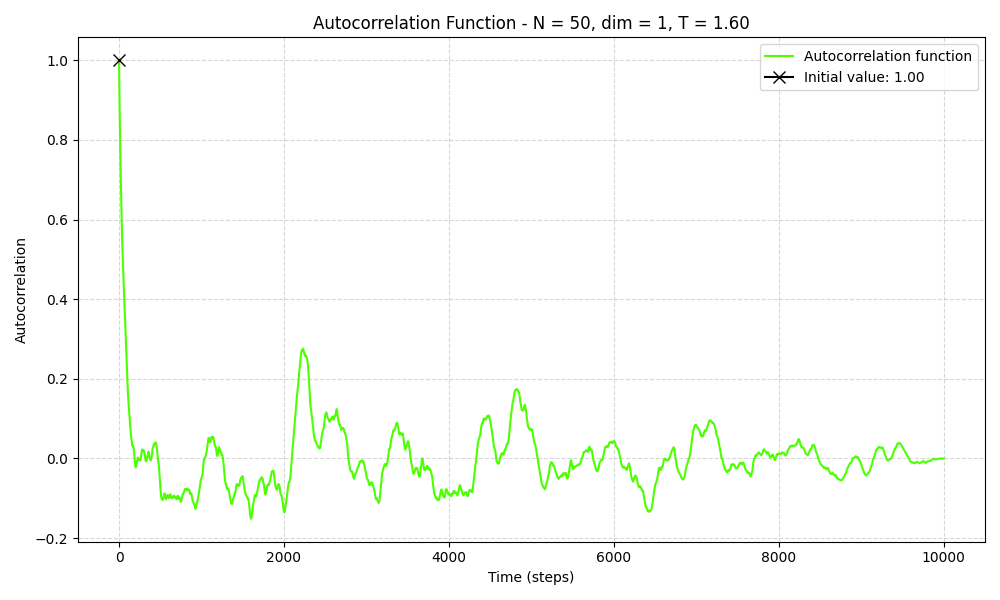
\includegraphics[width=1.\textwidth]{../pics_and_anims/autocorrelation_plot.png}
	\caption{Example of autocorrelation function for a Markov Chain.}
	\label{figure:autocorrelation_plot}
\end{figure}

[TODO: discussion of the autocorrelation function and its properties. An exponential fit after a certainb number of steps is only fitting noise.]

NOTA: Figure \ref{figure:autocorrelation_plot} prove the need of selecting a proper range to fit over. This is given by the linear portion of the following plot.

\begin{figure}[htbp]
	\centering
	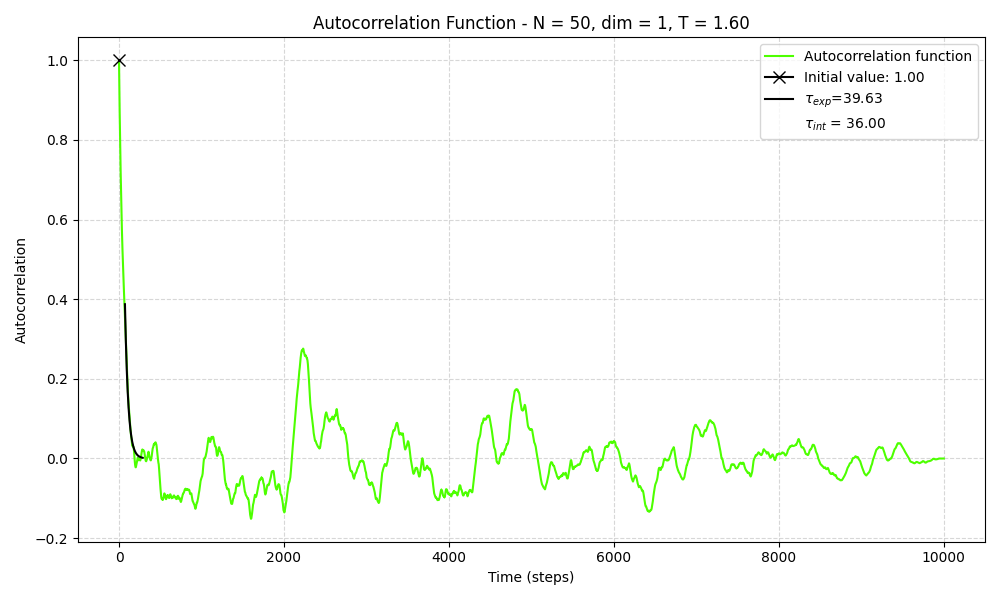
\includegraphics[width=1.\textwidth]{../pics_and_anims/autocorrelation_fit.png}
	\caption{Fitting to find $\tau_{exp}$.}
	\label{figure:autocorrelation_fit}
\end{figure}

[TODO: Didnt manage to make use of this]

\br

[TODO: discussion of Sokal's method]

\br

[TODO: discussion of the data blocking method]